We see that we have simplified the expectation value of \underline{one two-particle} operator (4 fermion operators) to a sum of products of \underline{two one-particle} propagators.
\[\begin{array}{r@{\;}c@{\;}l}
	\bra{\Phi_0}	& \multicolumn{2}{l}{T\big[c_{k_1,\sigma_1}(t_1)c_{k_2,\sigma_2}^\dagger(t_2)c_{k_3,\sigma_3}(t_3)c_{k_4,\sigma_4}^\dagger(t_4)\big]\ket{\Phi_0}}\\\\
					& =	& \phantom{+}i^2 G_0(k_1, t_1-t_2) G_0(k_3, t_3-t_4)\delta_{k_1,k_2}\delta_{k_3,k_4}\delta_{\sigma_1,\sigma_2}\delta_{\sigma_3,\sigma_4}\\\\
					&&-i^2 G_0(k_1, t_1-t_4) G_0(k_3, t_3-t_2) \delta_{k_1,k_4}\delta_{k_2,k_3}\delta_{\sigma_1,\sigma_4}\delta_{\sigma_2,\sigma_3}
\end{array}\]
As we will see, the expectation value of \underline{one} three-particle operator is reduced to a sum of products of \underline{three} one-particle propagators. \underline{Equivalently:} The expectation value of $N$-particle operator is reduced to a sum of products of $N/2$ one-particle propegators. The number of terms in the sum grows dramatically with $N$: $\sim (N/2)!$ (rough estimate).

We now go back to the second order expectation value. For the second order term we must look at the following contractions:
\[\begin{aligned}
    \text{1)}\qquad& \bra{\Phi_0}T\big[
\bcontraction[2ex]{}{c}{{}_{k,\sigma}(t)}{c}
\bcontraction[2ex]{c_{k,\sigma}(t)c_{k,\sigma}^\dagger(t')}{c}{{}_{k_1+q_1,\sigma_1}^\dagger(t_1)}{c}
\bcontraction[2ex]{c_{k,\sigma}(t)c_{k,\sigma}^\dagger(t')c_{k_1+q_1,\sigma_1}^\dagger(t_1)c_{k_1,\sigma_1}(t_1)}{c}{{}_{k_2+q_2,\sigma_2}^\dagger(t_2)}{c}
    c_{k,\sigma}(t)c_{k,\sigma}^\dagger(t')c_{k_1+q_1,\sigma_1}^\dagger(t_1)c_{k_1,\sigma_1}^{}(t_1)c_{k_2+q_2,\sigma_2}^\dagger(t_2)
c_{k_2,\sigma_2}(t_2)\big]\ket{\Phi_0}\\
    \text{2)}\qquad& \bra{\Phi_0}T\big[
\bcontraction[2ex]{}{c}{{}_{k,\sigma}(t)c_{k,\sigma}^\dagger(t')}{c}
\bcontraction[3ex]{c_{k,\sigma}(t)}{c}{{}_{k,\sigma}^\dagger(t')c_{k_1+q_1,\sigma_1}^\dagger(t_1)}{c}
\bcontraction[2ex]{c_{k,\sigma}(t)c_{k,\sigma}^\dagger(t')c_{k_1+q_1,\sigma_1}^\dagger(t_1)c_{k_1,\sigma_1}(t_1)}{c}{{}_{k_2+q_2,\sigma_2}^\dagger(t_2)}{c}
    c_{k,\sigma}(t)c_{k,\sigma}^\dagger(t')c_{k_1+q_1,\sigma_1}^\dagger(t_1)c_{k_1,\sigma_1}^{}(t_1)c_{k_2+q_2,\sigma_2}^\dagger(t_2)
c_{k_2,\sigma_2}(t_2)\big]\ket{\Phi_0}\\
    \text{3)}\qquad& \bra{\Phi_0}T\big[
\bcontraction[2ex]{}{c}{{}_{k,\sigma}(t)}{c}
\bcontraction[3ex]{c_{k,\sigma}(t)c_{k,\sigma}^\dagger(t')}{c}{{}_{k_1+q_1,\sigma_1}^\dagger(t_1)c_{k_1,\sigma_1}^{}(t_1)c_{k_2+q_2,\sigma_2}^\dagger(t_2)}{c}
\bcontraction[2ex]{c_{k,\sigma}(t)c_{k,\sigma}^\dagger(t')c_{k_1+q_1,\sigma_1}^\dagger(t_1)}{c}{{}_{k_1,\sigma_1}^{}(t_1)}{c}
    c_{k,\sigma}(t)c_{k,\sigma}^\dagger(t')c_{k_1+q_1,\sigma_1}^\dagger(t_1)c_{k_1,\sigma_1}^{}(t_1)c_{k_2+q_2,\sigma_2}^\dagger(t_2)
c_{k_2,\sigma_2}(t_2)\big]\ket{\Phi_0}\\
    \text{4)}\qquad& \bra{\Phi_0}T\big[
\bcontraction[2ex]{}{c}{{}_{k,\sigma}(t)c_{k,\sigma}^\dagger(t')}{c}
\bcontraction[3ex]{c_{k,\sigma}(t)}{c}{{}_{k,\sigma}^\dagger(t')c_{k_1+q_1,\sigma_1}^\dagger(t_1)c_{k_1,\sigma_1}^{}(t_1)c_{k_2+q_2,\sigma_2}^\dagger(t_2)}{c}
\bcontraction[2ex]{c_{k,\sigma}(t)c_{k,\sigma}^\dagger(t')c_{k_1+q_1,\sigma_1}^\dagger(t_1)}{c}{{}_{k_1,\sigma_1}^{}(t_1)}{c}
    c_{k,\sigma}(t)c_{k,\sigma}^\dagger(t')c_{k_1+q_1,\sigma_1}^\dagger(t_1)c_{k_1,\sigma_1}^{}(t_1)c_{k_2+q_2,\sigma_2}^\dagger(t_2)
c_{k_2,\sigma_2}(t_2)\big]\ket{\Phi_0}\\
    \text{5)}\qquad& \bra{\Phi_0}T\big[
\bcontraction[3ex]{}{c}{{}_{k,\sigma}(t)c_{k,\sigma}^\dagger(t')c_{k_1+q_1,\sigma_1}^\dagger(t_1)c_{k_1,\sigma_1}^{}(t_1)}{c}
\bcontraction[4ex]{c_{k,\sigma}(t)}{c}{{}_{k,\sigma}^\dagger(t')c_{k_1+q_1,\sigma_1}^\dagger(t_1)c_{k_1,\sigma_1}^{}(t_1)c_{k_2+q_2,\sigma_2}^\dagger(t_2)}{c}
\bcontraction[2ex]{c_{k,\sigma}(t)c_{k,\sigma}^\dagger(t')}{c}{{}_{k_1+q_1,\sigma_1}^\dagger(t_1)}{c}
    c_{k,\sigma}(t)c_{k,\sigma}^\dagger(t')c_{k_1+q_1,\sigma_1}^\dagger(t_1)c_{k_1,\sigma_1}^{}(t_1)c_{k_2+q_2,\sigma_2}^\dagger(t_2)
c_{k_2,\sigma_2}(t_2)\big]\ket{\Phi_0}\\
    \text{6)}\qquad& \bra{\Phi_0}T\big[
\bcontraction[4ex]{}{c}{{}_{k,\sigma}(t)c_{k,\sigma}^\dagger(t')c_{k_1+q_1,\sigma_1}^\dagger(t_1)c_{k_1,\sigma_1}^{}(t_1)}{c}
\bcontraction[2ex]{c_{k,\sigma}(t)}{c}{{}_{k,\sigma}^\dagger(t')c_{k_1+q_1,\sigma_1}^\dagger(t_1)}{c}
\bcontraction[3ex]{c_{k,\sigma}(t)c_{k,\sigma}^\dagger(t')}{c}{{}_{k_1+q_1,\sigma_1}^\dagger(t_1)c_{k_1,\sigma_1}^{}(t_1)c_{k_2+q_2,\sigma_2}^\dagger(t_2)}{c}
    c_{k,\sigma}(t)c_{k,\sigma}^\dagger(t')c_{k_1+q_1,\sigma_1}^\dagger(t_1)c_{k_1,\sigma_1}^{}(t_1)c_{k_2+q_2,\sigma_2}^\dagger(t_2)
c_{k_2,\sigma_2}(t_2)\big]\ket{\Phi_0}
\end{aligned}\]
This gives a sum of 6 terms, where each term is a product of three one-particle operators. The contracted operators must be placed together, and we therefore have to use the anti-commutation relations several times in order to get the correct sign for each term.
\[\begin{aligned}
    &\text{1:}\quad\\
&\bra{\Phi_0}T\big[c_{k,\sigma}(t)c_{k,\sigma}^\dagger(t')\big]\ket{\Phi_0}
\bra{\Phi_0}T\big[\underbrace{c_{k_1+q_1,\sigma_1}^\dagger(t_1)c_{k_1,\sigma_1}(t_1)}_{-c_{k_1,\sigma_1}(t_1)c_{k_1+q_1,\sigma_1}^\dagger(t_1)}\big]\ket{\Phi_0}
\bra{\Phi_0}T\big[\underbrace{c_{k_2+q_2,\sigma_2}^\dagger(t_2)c_{k_2,\sigma_2}(t_2)}_{-c_{k_2,\sigma_2}(t_2)c_{k_2+q_2,\sigma_2}^\dagger(t_2)}\big]\ket{\Phi_0}\\
&=\underline{(-1)^2 i^3 G_0(k,t-t') G_0(k_1,t_1-t_1) G_0(k_2, t_2-t_2) \delta_{k,k} \delta_{k_1+q_1,k_1} \delta_{k_2+q_2,k_2} \delta_{\sigma,\sigma} \delta_{\sigma_1,\sigma_1} \delta_{\sigma_2,\sigma_2}}
\end{aligned}\]

\[\begin{aligned}
    &\text{2:}\quad\\
&(-1)\bra{\Phi_0}T\big[c_{k,\sigma}(t)c_{k_1+q_1,\sigma_1}^\dagger(t_1)\big]\ket{\Phi_0}
\bra{\Phi_0}T\big[\underbrace{c_{k,\sigma}^\dagger(t')c_{k_1,\sigma_1}(t_1)}_{-c_{k_1,\sigma_1}(t_1)c_{k,\sigma}^\dagger(t')}\big]\ket{\Phi_0}
\bra{\Phi_0}T\big[\underbrace{c_{k_2+q_2,\sigma_2}^\dagger(t_2)c_{k_2,\sigma_2}(t_2)}_{-c_{k_2,\sigma_2}(t_2)c_{k_2+q_2,\sigma_2}^\dagger(t_2)}\big]\ket{\Phi_0}\\
&=\underline{(-1)^3 i^3 G_0(k,t-t_1) G_0(k,t_1-t') G_0(k_2, t_2-t_2) \delta_{k,k_1} \delta_{k,k_1+q_1} \delta_{k_2+q_2,k_2} \delta_{\sigma,\sigma_1} \delta_{\sigma,\sigma_1} \delta_{\sigma_2,\sigma_2}}
\end{aligned}\]

\[\begin{aligned}
    &\text{3:}\quad\\
&(-1)^2\bra{\Phi_0}T\big[c_{k,\sigma}(t)c_{k,\sigma}^\dagger(t')\big]\ket{\Phi_0}
\bra{\Phi_0}T\big[\underbrace{c_{k_1+q_1,\sigma_1}^\dagger(t_1)c_{k_2,\sigma_2}(t_2)}_{-c_{k_2,\sigma_2}(t_2)c_{k_1+q_1,\sigma_1}^\dagger(t_1)}\big]\ket{\Phi_0}
\bra{\Phi_0}T\big[c_{k_1,\sigma_1}(t_1)c_{k_2+q_2,\sigma_2}^\dagger(t_2)\big]\ket{\Phi_0}\\
&=\underline{(-1)^3 i^3 G_0(k,t-t') G_0(k_2,t_2-t_1) G_0(k_1, t_1-t_2)  \delta_{k_1+q_1,k_2} \delta_{k_2+q_2,k_1} \delta_{\sigma_1,\sigma_2}}
\end{aligned}\]

\[\begin{aligned}
    &\text{4:}\quad\\
&(-1)^3\bra{\Phi_0}T\big[c_{k,\sigma}(t)c_{k_1+q_1,\sigma_1}^\dagger(t_1)\big]\ket{\Phi_0}
\bra{\Phi_0}T\big[\underbrace{c_{k,\sigma}^\dagger(t')c_{k_2,\sigma_2}(t_2)}_{-c_{k_2,\sigma_2}(t_2)c_{k,\sigma}^\dagger(t')}\big]\ket{\Phi_0}
\bra{\Phi_0}T\big[c_{k_1,\sigma_1}(t_1)c_{k_2+q_2,\sigma_2}^\dagger(t_2)\big]\ket{\Phi_0}\\
&=\underline{i^3 G_0(k,t-t_1) G_0(k,t_2-t') G_0(k_1, t_1-t_2) \delta_{k,k_1+q_1} \delta_{k,k_2} \delta_{k_1,k_2+q_2} \delta_{\sigma,\sigma_2} \delta_{\sigma_1,\sigma_2} \delta_{\sigma,\sigma_1}}
\end{aligned}\]

\[\begin{aligned}
    &\text{5:}\quad\\
&(-1)^5\bra{\Phi_0}T\big[c_{k,\sigma}(t)c_{k_2+q_2,\sigma_2}^\dagger(t_2)\big]\ket{\Phi_0}
\bra{\Phi_0}T\big[\underbrace{c_{k,\sigma}^\dagger(t')c_{k_2,\sigma_2}(t_2)}_{-c_{k_2,\sigma_2}(t_2)c_{k,\sigma}^\dagger(t')}\big]\ket{\Phi_0}
\bra{\Phi_0}T\big[\underbrace{c_{k_1+q_1,\sigma_1}^\dagger(t_1)c_{k_1,\sigma_1}(t_1)}_{-c_{k_1,\sigma_1}(t_1)c_{k_1+q_1,\sigma_1}^\dagger(t_1)}\big]\ket{\Phi_0}\\
&=\underline{(-1) i^3 G_0(k,t-t_2) G_0(k,t_2-t') G_0(k_1, t_1-t_1) \delta_{k_1,k_1+q_1} \delta_{k,k_2+q_2} \delta_{k,k_2} \delta_{\sigma,\sigma_2} \delta_{\sigma,\sigma_2} \delta_{\sigma_1,\sigma_1}}
\end{aligned}\]

\[\begin{aligned}
    &\text{6:}\quad\\
&(-1)^4\bra{\Phi_0}T\big[c_{k,\sigma}(t)c_{k_2+q_2,\sigma_2}^\dagger(t_2)\big]\ket{\Phi_0}
\bra{\Phi_0}T\big[\underbrace{c_{k,\sigma}^\dagger(t')c_{k_1,\sigma_1}(t_1)}_{-c_{k_1,\sigma_1}(t_1)c_{k,\sigma}^\dagger(t')}\big]\ket{\Phi_0}
\bra{\Phi_0}T\big[\underbrace{c_{k_1+q_1,\sigma_1}^\dagger(t_1)c_{k_2,\sigma_2}(t_2)}_{-c_{k_2,\sigma_2}(t_2)c_{k_1+q_1,\sigma_1}^\dagger(t_1)}\big]\ket{\Phi_0}\\
&=\underline{i^3 G_0(k,t-t_2) G_0(k,t_1-t') G_0(k_2, t_2-t_1) \delta_{k,k_2+q_2} \delta_{k,k_1} \delta_{k_2,k_1+q_1} \delta_{\sigma,\sigma_2} \delta_{\sigma,\sigma_1} \delta_{\sigma_1,\sigma_2}}
\end{aligned}\]

We will now insert these terms into the double integral \underline{(NB: Equation reference)}. Remember that all six terms must be multiplied by $M_{q_1}$, $M_{q_2}$ and $iD_0(q_1,t_1-t_2)\delta_{q_1,-q_2}$. Finally we must sum over $k_1$, $k_2$, $q_1$, $q_2$, $\sigma_1$ and $\sigma_2$. Remember that
\[M_q = i\sqrt{\frac{\hbar}{2MN\omega_q}}\left(\vec{\xi}\cdot\vec{q}\right)\tilde{V}(\vec{q}) \rightarrow 0
\]
as $\vec{q}\rightarrow 0$. This means that three of the terms are zero:\\
\underline{First term}:
\[\begin{aligned}
    &\delta_{k_1+q_1,k_1} \delta_{k_2+q_2,k_2}\\
    \Rightarrow\quad &q_1 = q_2 = 0 \quad\Rightarrow \quad M_{q_1} = M_{q_2} = 0\\
    &\underline{\text{First term} = 0}
\end{aligned}\]
\underline{Second term}:
\[\begin{aligned}
    &\delta_{k_2+q_2,k_2}\\
    \Rightarrow\quad &q_2 = 0 \quad\Rightarrow \quad M_{q_2} = 0\\
    &\underline{\text{Second term} = 0}
\end{aligned}\]
\underline{Fifth term}:
\[\begin{aligned}
    &\delta_{k_1,k_1+q_1}\\
    \Rightarrow\quad &q_1 = 0 \quad\Rightarrow \quad M_{q_1} = 0\\
    &\underline{\text{Fifth term} = 0}
\end{aligned}\]
We have two $q$-summations, $\sum\limits_{q_1,q_2}$. However, since the free phonon-propagator is multiplied with $\delta_{q_1,-q_2}$, one of the summations is used to set $q_1 = -q_2$. Hence $M_{q_1}M_{q_2} = M_{q_1}M_{-q_1} = \left|M_{q_1}\right|^2$. For the remaining terms we then get:\\
\underline{Third term}:
\[\begin{aligned}
    &\delta_{k_1+q_1,k_2} \delta_{k_2+q_2,k_1} = \delta_{k_1+q_1,k_2} \delta_{k_2-q_1,k_1}\\
    \Rightarrow\quad &k_2 = k_1+q_1\\
    &\underline{\text{One $k$-summation left}}
\end{aligned}\]
\underline{Fourth term}:
\[\begin{aligned}
    &\delta_{k,k_1+q_1}\delta_{k,k_2} \delta_{k_1,k_2-q_1} = \delta_{k,k_2} \delta_{k_1,k_2-q_1}\\
    &\underline{\text{No $k$-summation}}
\end{aligned}\]
\underline{Sixth term}:
\[\begin{aligned}
    &\delta_{k,k_1}\delta_{k,k_2-q_1} \delta_{k_2,k_1+q_1} = \delta_{k,k_1} \delta_{k_2,k_1+q_1}\\
    &\underline{\text{No $k$-summation}}
\end{aligned}\]

Inserting these results we get
\[
\begin{aligned}
G(k,t-t') = &~\frac{G_0(k,t-t')}{\bra{\Phi_0}S(\infty,-\infty)\ket{\Phi_0}}\\
&+ \frac{(-i)^2}{2!}\frac{(-i)}{\bra{\Phi_0}S(\infty,-\infty)\ket{\Phi_0}}\sum_q \int\limits_{-\infty}^{\infty} \mathrm{d}t_1 \int\limits_{-\infty}^{\infty} \mathrm{d}t_2 \left|M_q\right|^2 i D_0(q,t_1-t_2) \\
&\times\sum_{\sigma_1,\sigma_2}\Big\{
\delta_{\sigma_1,\sigma_2}(-i)^3G_0(k,t-t')\sum_{k_1}G_0(k_1,t_1-t_2)G_0(k_1+q,t_2-t_1)\\
&+\delta_{\sigma,\sigma_1}\delta_{\sigma,\sigma_2}i^3G_0(k,t-t_1)G_0(k-q,t_1-t_2)G_0(k,t_2-t')\\
&+\delta_{\sigma,\sigma_1}\delta_{\sigma,\sigma_2}i^3 G_0(k,t-t_2)G_0(k,t_1-t')G_0(k+q,t_2-t_1)
\Big\}.
\end{aligned}
\]
In the third  term there is one spin summation left, while in the fourth and sixth terms the spin summations disappear. In order to give a diagrammatic representation of the previous equation, we define the following symbols for the propagators:

\begin{itemize}
    \item Free electron propagator: 
    \[G_0(k,t-t') = \qquad
\parbox{20mm}{\begin{feynman}{01G0}
    \begin{fmfgraph*}(110,5)
    \fmfleftn{i}{1}
    \fmfrightn{o}{1}
    \fmf{fermion,label=$k$}{i1,o1}
    \fmflabel{$t'$}{i1}
    \fmflabel{$t$}{o1}
    \end{fmfgraph*}
\end{feynman}}\]
    \item Free phonon propagator: \[D_0(q,t_1-t_2)=\qquad
\parbox{20mm}{\begin{feynman}{02D0}
    \begin{fmfgraph*}(110,5)
    \fmfleftn{i}{1}
    \fmfrightn{o}{1}
    \fmf{scalar,label=$q$}{i1,o1}
    \fmflabel{$t_2$}{i1}
    \fmflabel{$t_1$}{o1}
    \end{fmfgraph*}
\end{feynman}}\]
    \item Exact electron propagator: \[G(k,t-t') = \qquad
\parbox{20mm}{\begin{feynman}{03G}
    \begin{fmfgraph*}(110,5)
    \fmfleftn{i}{1}
    \fmfrightn{o}{1}
    \fmf{double_arrow,label=$k$}{i1,o1}
    \fmflabel{$t'$}{i1}
    \fmflabel{$t$}{o1}
    \end{fmfgraph*}
\end{feynman}}\]
\end{itemize}
Using this we get the diagrammatic representation of $G(k,t-t')$:
\[\begin{aligned}
&\parbox{40mm}{\begin{feynman}{04Gexpr}
    \begin{fmfgraph*}(110,20)
    \fmfleftn{i}{1}
    \fmfrightn{o}{1}
    \fmf{double_arrow,label=$k$}{i1,o1}
    \fmflabel{$t'$}{i1}
    \fmflabel{$t$}{o1}
    \end{fmfgraph*}
\end{feynman}} \qquad = \qquad
\parbox{40mm}{\begin{feynman}{05G0}
    \begin{fmfgraph*}(110,20)
    \fmfleftn{i}{1}
    \fmfrightn{o}{1}
    \fmf{fermion,label=$k$}{i1,o1}
    \fmflabel{$t'$}{i1}
    \fmflabel{$t$}{o1}
    \end{fmfgraph*}
\end{feynman}} \\
&+ \qquad \parbox{40mm}{\begin{feynman}{06G0}
    \begin{fmfgraph*}(110,20)
    \fmfleftn{i}{1}
    \fmfrightn{o}{1}
    \fmf{fermion,label=$k$}{i1,o1}
    \fmflabel{$t'$}{i1}
    \fmflabel{$t$}{o1}
    \end{fmfgraph*}
\end{feynman}}\quad\times \sum\limits_{k_1,q,\sigma_1}\qquad\quad
\parbox{40mm}{\begin{feynman}{073rd}
\begin{fmfgraph*}(110,30)
    \fmfleftn{i}{1}
    \fmfrightn{o}{1}
    \fmf{scalar, label=$q$}{i1,o1}
    \fmf{fermion, left=0.5, tension=.8, label=$k_1$}{i1,o1}
    \fmf{fermion, left=0.5, tension=.8, label=$k_1+q$}{o1,i1}
    \fmfdotn{i}{1}
    \fmfdotn{o}{1}
    \fmflabel{$t_2, M_q$}{i1}
    \fmflabel{$t_1, M_{-q}$}{o1}
    \end{fmfgraph*}
\end{feynman}}\qquad\qquad (-i)^3\\
&+ \qquad \parbox{120mm}{\begin{feynman}{084th}
\begin{fmfgraph*}(300,30)
    \fmfleftn{i}{1}
    \fmfrightn{o}{1}
    \fmf{fermion, label=$k$}{i1,v1}
    \fmf{fermion, label=$k-q$}{v1,v2}
    \fmf{fermion, label=$k$}{v2,o1}
    \fmf{scalar, left=0.8, tension=0, label=$q$}{v1,v2}
    \fmfdotn{v}{1}
    \fmfdotn{v}{2}
    \fmflabel{$t'$}{i1}
    \fmflabel{$t$}{o1}
    \fmfv{label=$t_2,, M_q$, l.a=-90}{v1}
    \fmfv{label=$t_1,, M_{-q}$, l.a=-90}{v2}
    \end{fmfgraph*}
\end{feynman}}\quad (i)^3\\
&+ \qquad \parbox{120mm}{\begin{feynman}{096th}
\begin{fmfgraph*}(300,30)
    \fmfleftn{i}{1}
    \fmfrightn{o}{1}
    \fmf{fermion, label=$k$}{i1,v1}
    \fmf{fermion, label=$k+q$}{v1,v2}
    \fmf{fermion, label=$k$}{v2,o1}
    \fmf{scalar, right=0.8, tension=0, label=$q$}{v2,v1}
    \fmfdotn{v}{1}
    \fmfdotn{v}{2}
    \fmflabel{$t'$}{i1}
    \fmflabel{$t$}{o1}
    \fmfv{label=$t_1,, M_q$, l.a=-90}{v1}
    \fmfv{label=$t_2,, M_{-q}$, l.a=-90}{v2}
    \end{fmfgraph*}
\end{feynman}}\quad (i)^3\\
& = \parbox{40mm}{\begin{feynman}{10g1}
\begin{fmfgraph*}(60,30)
    \fmfleftn{i}{1}
    \fmfrightn{o}{1}
    \fmf{fermion}{i1,o1}
    \end{fmfgraph*}
\end{feynman}} +
\underbrace{\parbox{30mm}{\begin{feynman}{11g2}
\begin{fmfgraph*}(60,30)
    \fmfleftn{i}{2}
    \fmfrightn{o}{2}
    \fmf{fermion}{i1,o1}
    \fmf{dashes}{i2,o2}
    \fmf{fermion,left=0.5}{i2,o2}
    \fmf{fermion,left=0.5}{o2,i2}
    \end{fmfgraph*}
\end{feynman}}}_{\text{Disconnected graph}} + ~~2 \times
\underbrace{\parbox{40mm}{\begin{feynman}{12g3}
\begin{fmfgraph*}(100,30)
    \fmfleftn{i}{1}
    \fmfrightn{o}{1}
    \fmf{fermion}{i1,v1}
    \fmf{fermion}{v1,v2}
    \fmf{fermion}{v2,o1}
    \fmf{dashes,left=1,tension=0}{v1,v2}
    \end{fmfgraph*}
\end{feynman}}}_{\text{Connected graph}}
\end{aligned}
\]
In general the correction to at each order consists of connected and disconnected graphs. The fourth and sixth terms give the same contribution, as seen by renaming the integration variables, $t_1 \leftrightarrow t_2$, $q\rightarrow -q$. This gives the connected graph to second order:
\[\begin{aligned}
    &\parbox{40mm}{\begin{feynman}{13g3}\begin{fmfgraph*}(100,30)
    \fmfleftn{i}{1}
    \fmfrightn{o}{1}
    \fmf{fermion}{i1,v1}
    \fmf{fermion}{v1,v2}
    \fmf{fermion}{v2,o1}
    \fmf{dashes,left=1,tension=0}{v1,v2}
    \end{fmfgraph*}\end{feynman}} \equiv F_2 \\
    =&~\frac{(-i)^2}{2!}\cdot 2(-i)i^3i \int\limits_{-\infty}^{\infty} dt_1 \int\limits_{-\infty}^{\infty} dt_2 \sum_q \left|M_q\right|^2 D_0(q, t_1-t_2)\\ &\times G_0(k, t-t_1) G_0(k-q, t_1-t_2) G_0(k, t_2- t') 
\end{aligned}\]
We see that the factor $1/2!$ is cancelled! For the unconnected graphs to second order we get:
\[\begin{aligned}
    &\parbox{30mm}{\begin{feynman}{14g2}\begin{fmfgraph*}(60,30)
    \fmfleftn{i}{2}
    \fmfrightn{o}{2}
    \fmf{fermion}{i1,o1}
    \fmf{dashes}{i2,o2}
    \fmf{fermion,left=0.5}{i2,o2}
    \fmf{fermion,left=0.5}{o2,i2}
    \end{fmfgraph*}\end{feynman}} = G_0F_1 \\
    F_1 =&  ~\frac{(-i)^2}{2!}\cdot (-i^3)(-i) \int\limits_{-\infty}^{\infty} dt_1 \int\limits_{-\infty}^{\infty} dt_2 \sum_q \left|M_q\right|^2 iD_0(q, t_1-t_2)\\
    & \times \sum_{k'} G_0(k'+q, t_2-t_1) G_0(k', t_1- t_2) 
\end{aligned}\]
Hence to second order we have:
\[G = \frac{1}{\bra{\Phi_0}S(\infty,-\infty)\ket{\Phi_0}}\left\{G_0(1+F_1) + F_2\right\}\]
But what about $\bra{\Phi_0}S(\infty,-\infty)\ket{\Phi_0}$? To second order (see exercise 5)
\[\bra{\Phi_0}S(\infty,-\infty)\ket{\Phi_0} = 1+F_1 = 1+ \parbox{25mm}{{\begin{feynman}{15F_1}\begin{fmfgraph*}(60,30)
    \fmfleftn{i}{1}
    \fmfrightn{o}{1}
    \fmf{dashes}{i1,o1}
    \fmf{fermion,left=0.5}{i1,o1}
    \fmf{fermion,left=0.5}{o1,i1}
    \end{fmfgraph*}\end{feynman}}}
\]
To higher orders one can \underline{always} write (we will not show the proof here, but it follows directly from Wick's theorem) 
\[\begin{aligned}
    &G = \frac{1}{\bra{\Phi_0}S(\infty,-\infty)\ket{\Phi_0}}\left\{G_0(1+F_1+A) + F_2(1+F_1+A) + B(1+F_1+A)\right\},\\
    &\bra{\Phi_0}S(\infty,-\infty)\ket{\Phi_0}=1+F_1+A,\\
    &\text{$A$: the sum of distinct higher order unconnected graphs},\\
    &\text{$B$: the sum of distinct higher order connected graphs.}
\end{aligned}
\]
Hence
\[\begin{aligned}
    &G= G_0 + F_2 + B\\
    &\parbox{120mm}{$B$: Contains graphs of 4th, 6th, 8th,... order in $M_q$. Terms of odd order in the electron-phonon vertex gives zero.}
\end{aligned}\]
We can now write
\[\begin{aligned}
    G(&{\bf{k}}, t-t') \\&= G_0({\bf{k}}, t-t') -i\sum\limits_{n=1}^{\infty} \frac{(-i)^n}{n!}\int\limits_{-\infty}^{\infty} dt_1...\int\limits_{-\infty}^{\infty} dt_n \underbrace{\bra{\Phi_0}T\left[c_{k\sigma}(t)c_{k\sigma}^\dagger(t')V(t_1)...V(t_n)\right] \ket{\Phi_0}_c}_{\text{Connected graphs}}\\
    &= G_0({\bf{k}}, t-t') -i\sum\limits_{n=1}^{\infty} (-i)^n\int\limits_{-\infty}^{\infty} dt_1...\int\limits_{-\infty}^{\infty} dt_n \underbrace{\bra{\Phi_0}T\left[c_{k\sigma}(t)c_{k\sigma}^\dagger(t')V(t_1)...V(t_n)\right] \ket{\Phi_0}_{dc}}_{\text{Distinct, connected graphs}}
\end{aligned}
\]
We have now achieved a considerable reduction of the number of contributions we need to calculate in the perturbation expansion, since there is far fewer connected graphs than the total number of graphs to each order. Similarily, the fraction of distinct connected graphs to each order is $1/n!$.

It is possible to further reduce the number of contributions we need to calculate: We introduce the Fourier-transformed Green's function
\[\begin{aligned}
    G(k,\omega) &= \int\limits_{-\infty}^{\infty} dt e^{i\omega t} G(k,t)\\
    G(k,t) &= \frac{1}{2\pi}\int\limits_{-\infty}^{\infty} d\omega e^{-i\omega t} G(k,\omega)\\
\end{aligned}\]
Exactly the same transformations are used for the phonon-propagators. To second order we have (with $t'=0$)
\[\begin{aligned}
    G(k,t) =&~ G_0(k,t) + i(-i) \int\limits_{-\infty}^{\infty} dt_1 \int\limits_{-\infty}^{\infty} dt_2 \sum_q \left|M_q\right|^2 iD_0(q, t_1-t_2) \\&\times G_0(k, t-t_1) G_0(k-q, t_1-t_2) G_0(k, t_2)
\end{aligned}
\]
Fourier-transforming the above, we get
\[\begin{aligned}
    G(k,\omega) = G_0(k, \omega) + &i(-i)\int\limits_{-\infty}^{\infty}dt_1\int\limits_{-\infty}^{\infty}dt_2 \sum_q \left|M_q\right|^2 \int\limits_{-\infty}^{\infty}dt~e^{i\omega t}\\
    &\times \frac{1}{2\pi}\int\limits_{-\infty}^{\infty} d\omega_1 D_0(q, \omega_1)e^{-i\omega_1(t_1-t_2)}\\
    &\times \frac{1}{2\pi}\int\limits_{-\infty}^{\infty} d\omega_2 G_0(k, \omega_2)e^{-i\omega_2(t-t_1)}\\
    &\times \frac{1}{2\pi}\int\limits_{-\infty}^{\infty} d\omega_3 G_0(k-q, \omega_3)e^{-i\omega_3(t_1-t_2)}\\
    &\times \frac{1}{2\pi}\int\limits_{-\infty}^{\infty} d\omega_4 G_0(k, \omega_4)e^{-i\omega_4t_2}\\
\end{aligned}\]
\[\begin{aligned}
    G(k,\omega) = &~G_0(k,\omega)\\ 
    &+ i\sum_q\left|M_q\right|^2 \int\limits_{-\infty}^{\infty} \frac{d\omega_1}{2\pi}... \int\limits_{-\infty}^{\infty} \frac{d\omega_4}{2\pi} iD_0(q, \omega_1) G_0(k,\omega_2) G_0(k-q,\omega_3)G_0(k,\omega_4)\\
    &\times \int\limits_{-\infty}^{\infty} dt_1~ e^{-it_1(\omega_1+\omega_2+\omega_3)} \cdot \int\limits_{-\infty}^{\infty} dt_2~ e^{-it_2(-\omega_1-\omega_3+\omega_4)} \cdot \int\limits_{-\infty}^{\infty} dt~ e^{it(\omega-\omega_2)}  
\end{aligned}\]
We use 
\[\int\limits_{-\infty}^{\infty} dt~ e^{it\omega} = 2\pi\delta(\omega)\]
which sets
\[\begin{aligned}
    \omega_2 &= \omega\\
    \omega_2 &= \omega_1+\omega_3\\
    \omega_4 &= \omega_1+\omega_3 = \omega_2 = \omega\\
    \omega_3 &= \omega_2-\omega_1 = \omega-\omega_1
\end{aligned}\]
We are then left with one $\omega_1$-integration,
\[\begin{aligned}
    G(k,\omega) = &~G_0(k,\omega)\\ 
    &+ i\sum_q\left|M_q\right|^2 \int\limits_{-\infty}^{\infty} \frac{d\omega_1}{2\pi} iD_0(q,\omega_1)G_0(k,\omega)G_0(k-q, \omega-\omega_1)G_0(k,\omega)\\
    =&~G_0(k,\omega) + G_0(k,\omega)\Sigma^{(2)}(k,\omega)G_0(k,\omega)
\end{aligned}\]
where
\[\begin{aligned}
    \Sigma^{(2)}(k,\omega) &= i\sum_q\left|M_q\right|^2\int\limits_{-\infty}^{\infty} \frac{d\omega_1}{2\pi} iD_0(q,\omega_1)G_0(k-q, \omega-\omega_1)\\
    &=\parbox{45mm}{\begin{feynman}{16Sigma(2)}\begin{fmfgraph*}(80,50)
    \fmfleftn{i}{1}
    \fmfrightn{o}{1}
    \fmf{dashes, left=0.8, tension=0, label=$q,,\omega_1$}{i1,o1}
    \fmf{fermion, label=$k-q,,\omega-\omega_1$}{i1,o1}
    \fmfv{label=$M_q$, l.a=-180}{i1}
    \fmfv{label=$M_{-q}$, l.a=-0}{o1}
    \fmfdotn{i}{1}
    \fmfdotn{o}{1}
    \end{fmfgraph*}\end{feynman}}
\end{aligned}\]
We have momentum and energy conservation at each vertex.

To second order we now have
\[\begin{aligned}
    G &= G_0 + G_0\Sigma^{(2)}G_0 + ...\\
     &=G_0(1+\Sigma^{(2)}G_0+...)\\
    G^{-1} &= G_0^{-1}(1-G_0\Sigma^{(2)})+...)\\
    &=G_0^{-1} - \Sigma^{(2)}+...
\end{aligned}\]

\subsection{The Dyson Equation}
We could have continued the perturbation expansion for $G$ and arrived at
\[\begin{aligned}
    G &= G_0 + G_0\Sigma^{(2)}G_0 + G_0\tilde{\Sigma}^{(4)}G_0 + ...\\
    &= G_0(1 + G_0\Sigma^{(2)} + G_0\tilde{\Sigma}^{(4)} + ...)\\
    G^{-1} &= G_0^{-1}(1 - G_0\Sigma^{(2)} - G_0\Sigma^{(4)} - ...)\\
    &=G_0^{-1} - (\Sigma^{(2)} + \Sigma^{(4)}+...)
\end{aligned}\]
From this we get
\begin{Indentskip}
    \[G^{-1} = G_0^{-1} - \Sigma \quad\qquad \text{(The Dyson equation)}\]
\end{Indentskip}
This is an exact expression for the Green's function.

The simplification is due to the fact that the perturbation expansion for $\Sigma$ is far simpler than the expansion for $G$!

\begin{Indentskip}
    $\Sigma:$ Is calculated from one-particle irreducible diagrams.
\end{Indentskip}

A one-particle irreducible diagram is a diagram which does not split into two pieces if one ''cuts'' a one-particle propagator.

\[G = G_0 + G_0\Sigma G_0 + G_0\Sigma G_0\Sigma G_0 + ...\]
We look at the fourth order terms:\\
One-particle reducible diagram:
\[
\left(\Sigma^{(2)}\right)^2G_0 = \parbox{50mm}{\begin{feynman}{17Sigma(2)2G0}\begin{fmfgraph*}(100,40)
    \fmfleftn{i}{1}
    \fmfrightn{o}{1}
    \fmf{dashes, left=1, tension=0}{i1,v1}
    \fmf{dashes, left=1, tension=0}{v2,o1}
    \fmf{fermion}{i1,v1}
    \fmf{fermion}{v1,v2}
    \fmf{fermion}{v2,o1}
    \fmfdotn{i}{1}
    \fmfdotn{o}{1}
    \fmfdotn{v}{1}
    \fmfdotn{v}{2}
    \end{fmfgraph*}\end{feynman}}
\]
One-particle irreducible fourth order graphs:
\[
    \Sigma_a^{(4)} = \parbox{40mm}{\begin{feynman}{18Sigma(4)a}\begin{fmfgraph*}(80,40)
    \fmfleftn{i}{2}
    \fmfrightn{o}{2}
    \fmf{dashes}{i1,i2}
    \fmf{dashes}{o1,o2}
    \fmf{fermion}{i1,o1}
    \fmf{fermion,left=0.5,tension=0}{i2,o2}
    \fmf{fermion,left=0.5,tension=0}{o2,i2}
    \fmfdotn{i}{1}
    \fmfdotn{o}{1}
    \fmfdotn{i}{2}
    \fmfdotn{o}{2}
    \end{fmfgraph*}\end{feynman}}\]
\[\Sigma_b^{(4)} = \parbox{45mm}{\begin{feynman}{19Sigma(4)b}\begin{fmfgraph*}(90,40)
    \fmfleftn{i}{1}
    \fmfrightn{o}{1}
    \fmf{dashes, left=0.8, tension=0}{i1,v2}
    \fmf{dashes, left=0.8, tension=0}{v1,o1}
    \fmf{fermion}{i1,v1}
    \fmf{fermion}{v1,v2}
    \fmf{fermion}{v2,o1}
    \fmfdotn{i}{1}
    \fmfdotn{o}{1}
    \fmfdotn{v}{1}
    \fmfdotn{v}{2}
    \end{fmfgraph*}\end{feynman}}\]
\[\Sigma_c^{(4)} = \parbox{45mm}{\begin{feynman}{20Sigma(4)c}\begin{fmfgraph*}(90,40)
    \fmfleftn{i}{1}
    \fmfrightn{o}{1}
    \fmf{dashes, left=0.8, tension=0}{i1,o1}
    \fmf{dashes, left=0.8, tension=0}{v1,v2}
    \fmf{fermion}{i1,v1}
    \fmf{fermion}{v1,v2}
    \fmf{fermion}{v2,o1}
    \fmfdotn{i}{1}
    \fmfdotn{o}{1}
    \fmfdotn{v}{1}
    \fmfdotn{v}{2}
    \end{fmfgraph*}\end{feynman}}
\]
We now use
\[\Sigma^{(4)} = \parbox{40mm}{\begin{feynman}{21Sigma(4)a}\begin{fmfgraph*}(80,40)
    \fmfleftn{i}{2}
    \fmfrightn{o}{2}
    \fmf{dashes}{i1,i2}
    \fmf{dashes}{o1,o2}
    \fmf{fermion}{i1,o1}
    \fmf{fermion,left=0.5,tension=0}{i2,o2}
    \fmf{fermion,left=0.5,tension=0}{o2,i2}
    \fmfdotn{i}{1}
    \fmfdotn{o}{1}
    \fmfdotn{i}{2}
    \fmfdotn{o}{2}
    \end{fmfgraph*}\end{feynman}}+
    \parbox{45mm}{\begin{feynman}{22Sigma(4)b}\begin{fmfgraph*}(90,40)
        \fmfleftn{i}{1}
        \fmfrightn{o}{1}
        \fmf{dashes, left=0.8, tension=0}{i1,v2}
        \fmf{dashes, left=0.8, tension=0}{v1,o1}
        \fmf{fermion}{i1,v1}
        \fmf{fermion}{v1,v2}
        \fmf{fermion}{v2,o1}
        \fmfdotn{i}{1}
        \fmfdotn{o}{1}
        \fmfdotn{v}{1}
        \fmfdotn{v}{2}
        \end{fmfgraph*}\end{feynman}}+
        \parbox{45mm}{\begin{feynman}{23Sigma(4)c}\begin{fmfgraph*}(90,40)
            \fmfleftn{i}{1}
            \fmfrightn{o}{1}
            \fmf{dashes, left=0.8, tension=0}{i1,o1}
            \fmf{dashes, left=0.8, tension=0}{v1,v2}
            \fmf{fermion}{i1,v1}
            \fmf{fermion}{v1,v2}
            \fmf{fermion}{v2,o1}
            \fmfdotn{i}{1}
            \fmfdotn{o}{1}
            \fmfdotn{v}{1}
            \fmfdotn{v}{2}
            \end{fmfgraph*}\end{feynman}}
    \]
in the Dyson equation to fourth order in $M_q$.
\begin{Indentskip}
    We see that the perturbation expansion for $G$ can be reduced to a perturbation expansion for $\Sigma$ with the help of the Dyson equation. This gives fewer contributions to consider.
\end{Indentskip}

We could have done the same thing for the phonon-propagator.
\[\begin{aligned}
    D(q,\omega) &= \parbox{45mm}{\begin{feynman}{24D}\begin{fmfgraph*}(90,10)
            \fmfleftn{i}{1}
            \fmfrightn{o}{1}
            \fmf{dbl_dashes_arrow, label=$q,,\omega$}{i1,o1}
            \end{fmfgraph*}\end{feynman}}\\
    D_0(q,\omega) &=\parbox{45mm}{\begin{feynman}{25D_0}\begin{fmfgraph*}(90,10)
            \fmfleftn{i}{1}
            \fmfrightn{o}{1}
            \fmf{dashes_arrow, label=$q,,\omega$}{i1,o1}
            \end{fmfgraph*}\end{feynman}}
\end{aligned}\]
The Dyson equation for the phonon-propagator reads
\begin{Indentskip}
    \[D^{-1}(q,\omega) = D_0^{-1} - \Pi\]
\end{Indentskip}
$\Pi(q,\omega)$ contains only irreducible one-phonon diagrams:
\[\begin{aligned}
    \parbox{40mm}{\begin{feynman}{26D}\begin{fmfgraph*}(90,10)
                \fmfleftn{i}{1}
                \fmfrightn{o}{1}
                \fmf{dbl_dashes_arrow, label=$q,,\omega$}{i1,o1}
                \end{fmfgraph*}\end{feynman}}
    &= \parbox{40mm}{\begin{feynman}{27D_0}\begin{fmfgraph*}(90,10)
            \fmfleftn{i}{1}
            \fmfrightn{o}{1}
            \fmf{dashes_arrow, label=$q,,\omega$}{i1,o1}
            \end{fmfgraph*}\end{feynman}} + \parbox{50mm}{\begin{feynman}{28D_term2}\begin{fmfgraph*}(120,30)
            \fmfleftn{i}{1}
            \fmfrightn{o}{1}
            \fmf{dashes_arrow}{i1,v1}
            \fmf{fermion, left=1}{v1,v2}
            \fmf{fermion, left=1}{v2,v1}
            \fmf{dashes_arrow}{v2,o1}
            \fmfdotn{v}{1}
            \fmfdotn{v}{2}
            \fmfv{label=$M_q$, l.a=120}{v1}
            \fmfv{label=$M_{-q}$, l.a=30}{v2}
            \end{fmfgraph*}\end{feynman}}\\
&+ \parbox{80mm}{\begin{feynman}{29D_term3}\begin{fmfgraph*}(160,30)
            \fmfleftn{i}{1}
            \fmfrightn{o}{1}
            \fmf{dashes}{i1,v1}
            \fmf{plain, left=0.8, tension=0.0}{v1,v2}
            \fmf{plain, left=0.8}{v2,v1}
            \fmf{dashes}{v2,v3}
            \fmf{plain, left=0.8, tension=0.0}{v3,v4}
            \fmf{plain, left=0.8}{v4,v3}
            \fmf{dashes}{v4,o1}
            \end{fmfgraph*}\end{feynman}} \\
&+ \parbox{45mm}{\begin{feynman}{30D_term4}\begin{fmfgraph*}(100,30)
            \fmfleftn{i}{1}
            \fmfrightn{o}{1}
            \fmf{dashes}{i1,v4}
            \fmf{dashes}{v1,o1}
            \fmf{plain, tension=1}{v1,v2}
            \fmf{plain, tension=0.2}{v2,v3}
            \fmf{plain, tension=1}{v3,v4}
            \fmf{dashes, left=1, tension=0.1}{v3,v2}
            \fmf{plain,right=1, tension=0.4}{v4,v1}
            \end{fmfgraph*}\end{feynman}} + \parbox{45mm}{\begin{feynman}{31D_term5}\begin{fmfgraph*}(100,30)
            \fmfleft{i}
            \fmfright{o}
            \fmftop{v2}
            \fmfbottom{v4}
            \fmf{dashes}{i,v1}
            \fmf{dashes}{v3,o}
            \fmf{plain,left=0.3}{v1,v2,v3}
            \fmf{plain,right=0.3}{v1,v4,v3}
            \fmf{dashes}{v2,v4}
            \end{fmfgraph*}\end{feynman}}
\end{aligned}\]
\[\Pi^{(2)} = \parbox{30mm}{\begin{feynman}{32Pi(2)}\begin{fmfgraph*}(60,30)
            \fmfleft{i}
            \fmfright{o}
            \fmf{fermion, left=0.5}{i,o}
            \fmf{fermion, left=0.5}{o,i}
            \end{fmfgraph*}\end{feynman}}\qquad\quad \text{Irreducible}\]
\[\Pi^{(4)}_a = \parbox{30mm}{\begin{feynman}{33Pi(4)_a}\begin{fmfgraph*}(60,30)
            \fmfleft{i}
            \fmfright{o}
            \fmf{plain, left=0.8, tension=0.0}{i,v1}
            \fmf{plain, left=0.8}{v1,i}
            \fmf{dashes}{v1,v2}
            \fmf{plain, left=0.8, tension=0.0}{v2,o}
            \fmf{plain, left=0.8}{o,v2}
            \end{fmfgraph*}\end{feynman}}\qquad\quad \text{Reducible}\]
\[\Pi^{(4)}_b = \parbox{30mm}{\begin{feynman}{34Pi(4)_b}\begin{fmfgraph*}(60,30)
                        \fmfleft{i}
                        \fmfright{o}
                        \fmf{plain, tension=1}{i,v1}
                        \fmf{plain, tension=0.2}{v1,v2}
                        \fmf{plain, tension=1}{v2,o}
                        \fmf{dashes, right=1, tension=0.1}{v2,v1}
                        \fmf{plain,left=1, tension=0.4}{o,i}
                        \end{fmfgraph*}\end{feynman}}\qquad\quad \text{Irreducible}\]
\[\Pi^{(4)}_c = \parbox{30mm}{\begin{feynman}{35Pi(4)_c}\begin{fmfgraph*}(60,30)
                        \fmfleft{i}
                        \fmfright{o}
                        \fmftop{v1}
                        \fmfbottom{v2}
                        \fmf{plain,left=0.25}{i,v1,o}
                        \fmf{plain,right=0.25}{i,v2,o}
                        \fmf{dashes}{v1,v2}
                        \end{fmfgraph*}\end{feynman}}\qquad\quad \text{Irreducible}\]
How did we get the diagrams for $\Pi$? We used the \underline{Feynman rules}: For diagrams of order $2m$
\begin{enumerate}
    \item Draw all topologically distinct diagrams with $2m$ vertices
    \begin{feynman}{36Vertex}\begin{fmfgraph*}(60,60)
                            \fmfleftn{i}{2}
                            \fmfright{o}
                            \fmf{fermion}{i1,v1,i2}
                            \fmf{dashes}{v1,o}
                            \fmfdot{v1}
                            \fmfv{label=$M_q$, l.a=40}{v1}
    \end{fmfgraph*}\end{feynman}
    To every vertex, we associate a factor $M_q$.
    \item With every free electron line, we associate a factor
    \[G_0(k,\omega) = \parbox{30mm}{\begin{feynman}{37G0Feynman}\begin{fmfgraph*}(40,10)
                            \fmfleft{i}
                            \fmfright{o}
                            \fmf{fermion,label=$k,,\omega$}{i,o}
                            \fmfv{label=$\alpha$, l.a=90}{i}
                            \fmfv{label=$\beta$, l.a=90}{o}
    \end{fmfgraph*}\end{feynman}} = \frac{\delta_{\alpha\beta}}{\omega-\epsilon_k + i \delta_k}\]
    where $\delta_k = \delta \mathrm{sign}(\epsilon_k-\mu)$. This is a combined particle and hole propagator.
    \item With each phonon line we associate a factor
    \[D_0(q,\omega) = \parbox{30mm}{\begin{feynman}{38D0Feynman}\begin{fmfgraph*}(60,10)
                            \fmfleft{i}
                            \fmfright{o}
                            \fmf{scalar,label=$q,,\omega$}{i,o}
    \end{fmfgraph*}\end{feynman}} = \frac{2\omega_q}{\omega^2-\omega_q^2 + i \delta}.\]
    \item Make sure that momentum and energy is conserved at each vertex.
    \item Prefactor for each distinct diagram:
    \[\begin{aligned}
        &i^m(-1)^F(2s+1)^F\\
        &\text{$s:$ spinn ($= 1/2$ for electrons)}\\
        &\text{$F:$ the number of closed fermion loops in the diagram:} \parbox{30mm}{\begin{feynman}{39closed_loop}\begin{fmfgraph*}(60,20)
            \fmfleft{i}
            \fmfright{o}
            \fmf{fermion, left=0.5}{i,o}
            \fmf{fermion, left=0.5}{o,i}
            \end{fmfgraph*}\end{feynman}}\\
        & \text{\underline{NB}: this is not a closed loop:} \parbox{30mm}{\begin{feynman}{40not_closed_loop}\begin{fmfgraph*}(60,20)
            \fmfleft{i}
            \fmfright{o}
            \fmf{fermion, left=0.5}{i,o}
            \fmf{fermion, right=0.5}{i,o}
            \end{fmfgraph*}\end{feynman}} 
    \end{aligned}\]
    \item Integrate over independent momenta and frequencies.
\end{enumerate}

\subsection*{Examples}
\paragraph{$\Sigma$ to Second order in $M_q$}
The diagram is
\begin{feynman}{41example1}\begin{fmfgraph*}(160,40)
            \fmfleft{i}
            \fmfright{o}
            \fmf{fermion,label=$k,,\omega$}{i,v1}
            \fmf{fermion,label=$k-q,,\omega-\omega_1$}{v1,v2}
            \fmf{fermion,label=$k,,\omega$}{v2,o}
            \fmf{dashes, left=0.8, tension=0.0, label=$q,,\omega_1$}{v1,v2}
            \fmfdotn{v}{2}
\end{fmfgraph*}\end{feynman}
which yields
\[\Sigma^{(2)}(k,\omega) = i\sum_q\int\limits_{-\infty}^{\infty}\frac{d \omega_1}{2\pi}\left|M_q\right|^2D_0(q,\omega_1)G_0(k-q,\omega-\omega_1)\]

\paragraph{$\Pi$ to Second order in $M_q$}
The diagram is
\begin{feynman}{42example2}\begin{fmfgraph*}(160,40)
            \fmfleft{i}
            \fmfright{o}
            \fmf{scalar,label=$q,,\omega$}{i,v1}
            \fmf{scalar,label=$q,,\omega$}{v2,o}
            \fmf{fermion, label=$k_1+q,,\omega+\omega_1$, left=0.8}{v1,v2}
            \fmf{fermion, label=$k_1,,\omega_1$, left=0.8}{v2,v1}
            \fmfdotn{v}{2}
\end{fmfgraph*}\end{feynman}
which yields
\[\Pi^{(2)}(q,\omega) = i(-1)^1 \left(2\cdot\frac{1}{2}+1\right) \sum_{k_1}\int\limits_{-\infty}^{\infty}\frac{d \omega_1}{2\pi}\left|M_q\right|^2G_0(k_1,\omega_1)G_0(k_1-q,\omega+\omega_1),\]
where $\left|M_q\right|^2$ can be moved outside the sum and integration. The advantage here is that the diagrams can be given a physical interpretation, in contrast to the associated mathematical expressions. Let's look at a more complicated example.

\[\parbox{60mm}{
\begin{feynman}{43example3}\begin{fmfgraph*}(160,40)
    \fmftop{v0,v2,v3,v5}
    \fmfbottom{i,v1,v4,o}
    \fmf{fermion}{i,v1,v4,o}
    \fmf{scalar}{v1,v2}
    \fmf{scalar}{v3,v4}
    \fmf{fermion, left=0.6, tension=0.2}{v2,v3,v2}
\end{fmfgraph*}\end{feynman}} \sim |M|^4 \qquad \text{Fourth order}\]
The diagram describes an electron which comes in, excites a phonon and continues to propagate as a free electron. However, the phonon does \underline{not} propagate freely, it excites a particle-hole excitation along its way. Finally, the phonon and electron collide. Therefore, the process is a version of
\[\parbox{50mm}{\begin{feynman}{44example4}\begin{fmfgraph*}(140,40)
    \fmftop{v0,v2,v5}
    \fmfbottom{i,v1,v4,o}
    \fmf{fermion}{i,v1,v4,o}
    \fmf{scalar,left=0.3}{v1,v2}
    \fmf{scalar,left=0.3}{v2,v4}
    \fmfblob{20}{v2}
\end{fmfgraph*}\end{feynman}} = \parbox{50mm}{\begin{feynman}{45example5}\begin{fmfgraph*}(140,40)
    \fmfleft{i}
    \fmfright{o}
    \fmf{double_arrow}{i,v1,v2,o}
    \fmf{boson,left=1, tension=0.2}{v1,v2}
\end{fmfgraph*}\end{feynman}}\]
where the blob indicates that something happens with the phonon. We here see the traces of complicated effects. Let's look at the above diagram in more detail, where $m=2$, $F=1$:
\[\parbox{100mm}{
\begin{feynman}{46example6}\begin{fmfgraph*}(200,60)
    \fmftop{v0,v2,v3,v5}
    \fmfbottom{i,v1,v4,o}
    \fmf{fermion,label=$k,,\omega$}{i,v1}
    \fmf{fermion,label=$k-q,,\omega-\omega_1$}{v1,v4}
    \fmf{fermion,label=$k,,\omega$}{v4,o}
    \fmf{scalar,label=$q_1,,\omega_1$,label.side=left}{v1,v2}
    \fmf{scalar,label=$g_1,,\omega_1$,label.side=left}{v3,v4}
    \fmf{fermion, left=0.6, tension=0.2, label=$k_2,,\omega_2$}{v3,v2}
    \fmf{fermion, left=0.6, label=$k_2+q_1,,\omega_2+\omega_1$}{v2,v3}
\end{fmfgraph*}\end{feynman}} \sim |M|^4\]
From this we get the mathematical expression
\[\begin{aligned}
    &i^2(-1)^1\left(2\cdot\frac{1}{2}+1\right)^1G_0(k,\omega)^2 \sum_{q_1}\sum_{k_2} \int \limits_{-\infty}^{\infty} \frac{d \omega_1}{2\pi}\int \limits_{-\infty}^{\infty} \frac{d \omega_2}{2\pi} \left|M_{q_1}\right|^4 \\
    &\times D_0(q_1,\omega_1)^2 G_0(k_2,\omega_2)G_0(k-q_1,\omega-\omega_1)G_0(k_2+q_1,\omega_1+\omega_2)
\end{aligned}\]
We here see that the expressions quickly become complicated.
\begin{enumerate}[i)]
    \item Small quantitative changes $\Rightarrow$ use perturbation theory to low order (second order).
    \item If we expect large changes, we can sum classes of simple () diagrams.
\end{enumerate}
Example:
    \[\begin{aligned}
        G &\approx \parbox{25mm}{\begin{feynman}{47Gapprox1}\begin{fmfgraph*}(50,20)
        \fmfleft{i}
        \fmfright{o}
        \fmf{fermion}{i,o}
    \end{fmfgraph*}\end{feynman}} + 
\parbox{35mm}{\begin{feynman}{48Gapprox2}\begin{fmfgraph*}(80,20)
        \fmfleft{i}
        \fmfright{o}
        \fmf{fermion}{i,v1,v2,o}
        \fmf{dashes,left=1,tension=0.1}{v1,v2}
    \end{fmfgraph*}\end{feynman}} +  \parbox{45mm}{\begin{feynman}{49Gapprox3}\begin{fmfgraph*}(120,20)
        \fmfleft{i}
        \fmfright{o}
        \fmf{fermion}{i,v1,v2,v3,v4,o}
        \fmf{dashes,left=1,tension=0.1}{v1,v2}
        \fmf{dashes,left=1,tension=0.1}{v3,v4}
    \end{fmfgraph*}\end{feynman}} + ...\\
    &= G_0 \left(1+\Sigma^{(2)}G_0 + (\Sigma^{(2)}G_0)^2+...\right)\\
    &= \frac{G_0}{1-G_0\Sigma^{(2)}} = \frac{1}{G_0^{-1}-\Sigma^{(2)}}
    \end{aligned}\]
We use
\[\begin{aligned}
        G_0(k,\omega) &= \frac{\theta(\epsilon_k-\epsilon_F)}{\omega-\epsilon_k+i\delta} + \frac{\theta(\epsilon_F-\epsilon_k)}{\omega-\epsilon_k-i\delta} \\
        & = \frac{1}{\omega - \epsilon_k +i\delta_k}\\
        \delta_k & = \delta \mathrm{sign}(\epsilon_k-\epsilon_F)
    \end{aligned}\]
    to get an approximate expression for $G$,
    \[\begin{aligned}
        G(k,\omega) &\approx \frac{1}{\omega-\epsilon_k + i\delta_k - \Sigma^{(2)}}\\
        \Sigma^{(2)} &= \Sigma^{(2)}_R + i\Sigma^{(2)}_I
\end{aligned}\]
\begin{Indentskip}
    \[G = \frac{1}{\omega - \tilde{\epsilon}_k+i/\tau}\]
    \[\tilde{\epsilon}_k = \epsilon_k + \Sigma^{(2)}_R\]
    \[\tau^{-1} = - \Sigma^{(2)}_I\]
\end{Indentskip}
From this we see that $G_0 \sim \exp(-i\epsilon_k t - \delta t)$, while $G_0 \sim \exp(-i\tilde{\epsilon}_k t - t/\tau)$. This means that $\Sigma^{(2)}_R$ \underline{renormalizes} the energy, $\epsilon_k \rightarrow \tilde{\epsilon}_k$, while $\Sigma^{(2)}_I$ leads to a \underline{damping} due to the spreading of plane waves.

\subsection{Effective Interaction Between Electrons due to Phonons}
\[V = \sum_{kq\sigma} M_q \left(a_{-q}^\dagger + a_q\right)c_{k+q,\sigma}^\dagger c_{k,\sigma}\]
This is a scattering process which gives rise to
\[\parbox{60mm}{\begin{feynman}{50Vertex}\begin{fmfgraph*}(60,40)
    \fmfleftn{i}{2}
    \fmfright{o}
    \fmf{fermion}{i1,v1,i2}
    \fmf{dashes}{v1,o}
    \fmfdot{v1}
    \fmfv{label=$M_q$, l.a=40}{v1}
\end{fmfgraph*}\end{feynman}}\qquad\quad\text{Electron-phonon interaction}\]
which we call a \underline{vertex}. This gives rise to a electron-phonon-electron interaction, or alternatively: An effective interaction between two electrons mediated by phonons.\\
\underline{Classical picture:}
\[\begin{aligned}
&\text{i)}\qquad\parbox{40mm}{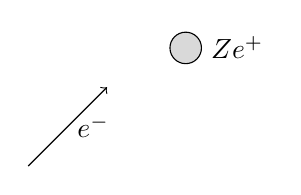
\begin{tikzpicture}
    \draw[->] (0,0) -- node[anchor=west] {$e^{-}$} ++ (1,1);
    \draw[fill=gray!30] (2,1.5) node[anchor=west, right=2mm] {$Ze^{+}$} circle (2mm);
    \end{tikzpicture}} \Rightarrow \qquad\text{ii)}\parbox{40mm}{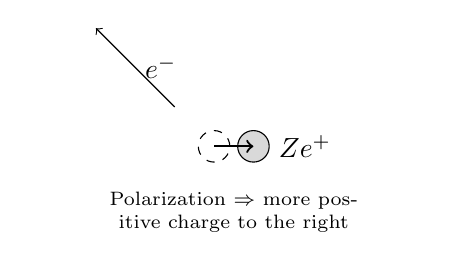
\begin{tikzpicture}
    \draw[->] (1,0.5) -- node[anchor=west] {$e^{-}$} (0,1.5);
    \draw[fill=gray!30] (2,0) node[anchor=west, right=2mm] {$Ze^{+}$} circle (2mm);
    \draw[dashed] (1.5,0) circle (2mm);
    \draw[thick,->] (1.5,0) -- node [align=center,text width=5cm,midway,anchor=north,yshift=-3ex,font=\scriptsize] {Polarization $\Rightarrow$ more positive charge to the right} (2,0);   
    \end{tikzpicture}}\\
\Rightarrow\quad&\text{iii)}\qquad\parbox{40mm}{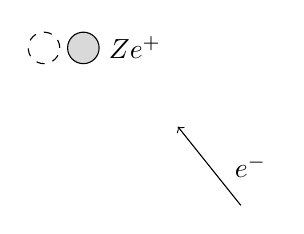
\begin{tikzpicture}
    \draw[fill=gray!30] (0.5,0) node[anchor=west, right=2mm] {$Ze^{+}$} circle (2mm);
    \draw[dashed] (0,0) circle (2mm);
    \draw[->] (2.5,-2) -- node[anchor=west, right=2mm] {$e^{-}$} (1.7,-1);
    \end{tikzpicture}} \qquad \qquad \parbox{36mm}{\footnotesize Attracts another electron because it ''sees'' the little extra positive charge}
\end{aligned}\]
